\documentclass[usenames,dvipsnames, 18pt, compress, aspectratio=169]{beamer}

% can be compiled by xelatex -shell-escape presentation.tex
% lualatex -shell-escape presentation.tex

\usetheme[]{metropolis}

\usepackage[utf8]{inputenc}
\usepackage[russian, english]{babel}
\usepackage{booktabs}
\usepackage[scale=2]{ccicons}
\usepackage{listings}
\usepackage{marvosym}
\usepackage{color}
\usepackage{xcolor}
\usepackage[document]{ragged2e}
\usepackage[export]{adjustbox}
\usepackage{fontawesome}
\usepackage{enumitem}
\usepackage{minted}
\usemintedstyle{tango}
\usepackage[normalem]{ulem}
\usepackage{tikz}
\usetikzlibrary{patterns}
\usetikzlibrary{mindmap}
\usetikzlibrary{shapes.misc, fit}
\usepackage{graphicx}
\usepackage{eso-pic}
\usepackage{verbatim}
\usepackage{smartdiagram}
\usesmartdiagramlibrary{additions}
\usetikzlibrary{trees}
\usepackage{datetime}
\usepackage{hyperref}

\usepackage{tcolorbox}
\usepackage{tabularx}
\usepackage{array}
\usepackage{colortbl}
\tcbuselibrary{skins}

\usetikzlibrary{shapes,arrows,positioning}
\graphicspath{{images/}}
\newfontfamily{\FA}{FontAwesome}

\def\twitter{{\FA \faTwitter}}
\def\github{{\FA \faGithub}}
\def\email{{\FA \faEnvelope}}

\renewcommand{\ttdefault}{pcr}
\newfontfamily{\ttfamily}{Fira Code}

\usefonttheme{professionalfonts} % using non standard fonts for beamer
\usefonttheme{serif} % default family is serif
\usepackage{fontspec}
\setmainfont{Liberation Sans}
\newfontfamily\ExtraLight{Liberation Sans}
\newfontfamily\Light{Liberation Sans}
\newfontfamily\Book{Liberation Sans}
\newfontfamily\Medium{Liberation Sans}

\makeatletter
\newcommand\HUGE{\@setfontsize\Huge{32}{41}}
\makeatother

\newcommand\AtPagemyUpperLeft[1]{\AtPageLowerLeft{%
\put(\LenToUnit{0.85\paperwidth},\LenToUnit{0.05\paperheight}){#1}}}

\newcommand\AtPagemyUpperTop[1]{\AtPageLowerLeft{%
\put(\LenToUnit{0.42\paperwidth},\LenToUnit{0.90\paperheight}){#1}}}

\renewcommand{\ULthickness}{2.0pt}

\definecolor{links}{HTML}{0099FF}
\hypersetup{colorlinks, linkcolor=, urlcolor=links}
\definecolor{greenGood}{HTML}{99FF99}
\definecolor{redBad}{HTML}{FF9980}

\setbeamerfont{section title}{family=\Book, size=\Huge, shape=\normalfont}
\setbeamerfont{frametitle}{family=\Book, size=\large, shape=\normalfont}
\setbeamerfont{title}{family=\Book, size=\Large, shape=\normalfont}
\setbeamerfont{subtitle}{size=\small}
\setbeamerfont{author}{family=\ExtraLight, size=\footnotesize}

\definecolor{cec1d24}{RGB}{236,29,36}
\definecolor{cffffff}{RGB}{255,255,255}

\pagenumbering{gobble}

\newdateformat{specialdate}{\twodigit{\THEDAY}-\twodigit{\THEMONTH}-\THEYEAR}

\newcommand\tikzmark[1]{%
  \tikz[overlay,remember picture] \coordinate (#1);}

\setbeamertemplate{title page}
{

  \vspace*{2.1cm}
  \begin{minipage}[b][\paperheight]{\textwidth}
  \begin{center}

    \ifx\inserttitle\@empty\else
    {{% \inserttitle is nonempty
      \raggedright%
      %\linespread{1.0}%
      \usebeamerfont{title}%
      \usebeamercolor[fg]{title}%
      %\vspace*{1.3em}
      \if@noSmallCapitals%
        \inserttitle%
      \else%
        \scshape{\color{black} \textbf{\begin{center}\inserttitle\end{center}}}%
      \fi%
      \vspace*{0.3em}
    }}
    \fi

    \vspace*{0.5em}%

    \ifx\insertsubtitle\@empty\else
    {{% \insertsubtitle is nonempty
      \usebeamerfont{subtitle}%
      \usebeamercolor[fg]{subtitle}%
      {\color{black} \insertsubtitle}%
      \vspace*{3.0em}%
    }}
    \fi

    \vspace*{1.0em}%

    \usebeamerfont{author}%
    \usebeamercolor[fg]{author}%
    {\color{black} \insertauthor}%

    \vspace*{1.5em}
    \fontsize{8pt}{10}\selectfont
    {\color{black} 03-12-2019}%

    \vfill
    \vspace*{2em}
  \end{center}
  \end{minipage}
}

\setbeamertemplate{section page}
{
  \vspace{2em}
  \centering
  \begin{minipage}{22em}
    \usebeamercolor[fg]{section title}
    \usebeamerfont{section title}
    {\color{black} \insertsectionhead\\[-1ex]}
  \end{minipage}
  \par
}

\setbeamertemplate{footline}
{
\begin{beamercolorbox}[wd=\textwidth,ht=3ex,dp=3ex,leftskip=0.3cm,rightskip=0.3cm]{structure}
  \usebeamerfont{page number in head/foot}
  \insertframenumber
\end{beamercolorbox}
}

\title{Modern BTree\\ techniques}
\subtitle{}
\date{\today}
\author{DMITRY DOLGOV}
\institute{}

\tikzset{rum-node/.style={draw,circle,fill=white,minimum width=2cm}}
\tikzset{rum-extra-node/.style={rectangle, draw, dashed, rounded corners, fill=white }}
\tikzset{btree-key/.style={minimum height=1cm, pattern=north west lines, draw}}
\tikzset{btree-pointer/.style={minimum height=1cm, draw}}
\tikzset{btree-hide/.style={draw opacity=0, line width=0, pattern=none}}
\tikzset{btree-leaf/.style={fill=greenGood}}
\tikzset{btree-branch/.style={fill=gray!20}}
\tikzset{btree-line/.style={line width=0.5pt}}
\tikzset{btree-path/.style={btree-pointer, minimum width=0.8cm, fill=red, opacity=0.5}}
\tikzset{>=latex}

\newcommand{\btreenode}[5] {
    \path
      node[btree-pointer, #2, #3] (pointer1#1) {}
      node[btree-key, right=0 of pointer1#1, #3] (sep1#1) {}
      node[btree-key, left=0 of pointer1#1, #3] (sep2#1) {}
      node[btree-pointer, right=0 of sep1#1, #3] (pointer2#1) {}
      node[btree-pointer, left=0 of sep2#1, #3] (pointer3#1) {}
      node[btree-key, right=0 of pointer2#1, #3] (sep3#1) {}
      node[btree-key, left=0 of pointer3#1, #3] (sep4#1) {}
      node[draw, inner sep=0, behind path, #4,
          fit=(pointer1#1)(pointer2#1)(pointer3#1)
              (sep1#1)(sep2#1)(sep3#1)(sep4#1)
      ] (node#1) {};

      \ifthenelse{ \equal{#5}{show-pointers} } {
            \coordinate[below=0.5 of pointer1#1] (heap-pointer1#1);
            \coordinate[below=0.5 of pointer2#1] (heap-pointer2#1);
            \coordinate[below=0.5 of pointer3#1] (heap-pointer3#1);

            \draw[->, btree-line] (pointer1#1.south) -- (heap-pointer1#1.north);
            \draw[->, btree-line] (pointer2#1.south) -- (heap-pointer2#1.north);
            \draw[->, btree-line] (pointer3#1.south) -- (heap-pointer3#1.north);
      } {}
}

\begin{document}
{
  \usebackgroundtemplate{
\includegraphics[width=\paperwidth]{template_2.png}}%
  \fontsize{17pt}{18}\selectfont
  \maketitle
}

\AddToShipoutPictureBG{
  \AtPagemyUpperLeft{{
\includegraphics[width=2.0cm,keepaspectratio]{logo.png}}}
}%

\setbeamertemplate{background canvas}{
\begin{tikzpicture}
    \clip (0,0) rectangle (\paperwidth,\paperheight);
    \fill[color=orange] (4cm, \paperheight-6pt) rectangle (\paperwidth-4cm,\paperheight);
\end{tikzpicture}
}

\fontsize{17pt}{18}\selectfont

\begin{frame}
    \frametitle{}
    \begin{center}
        \only<1>{
            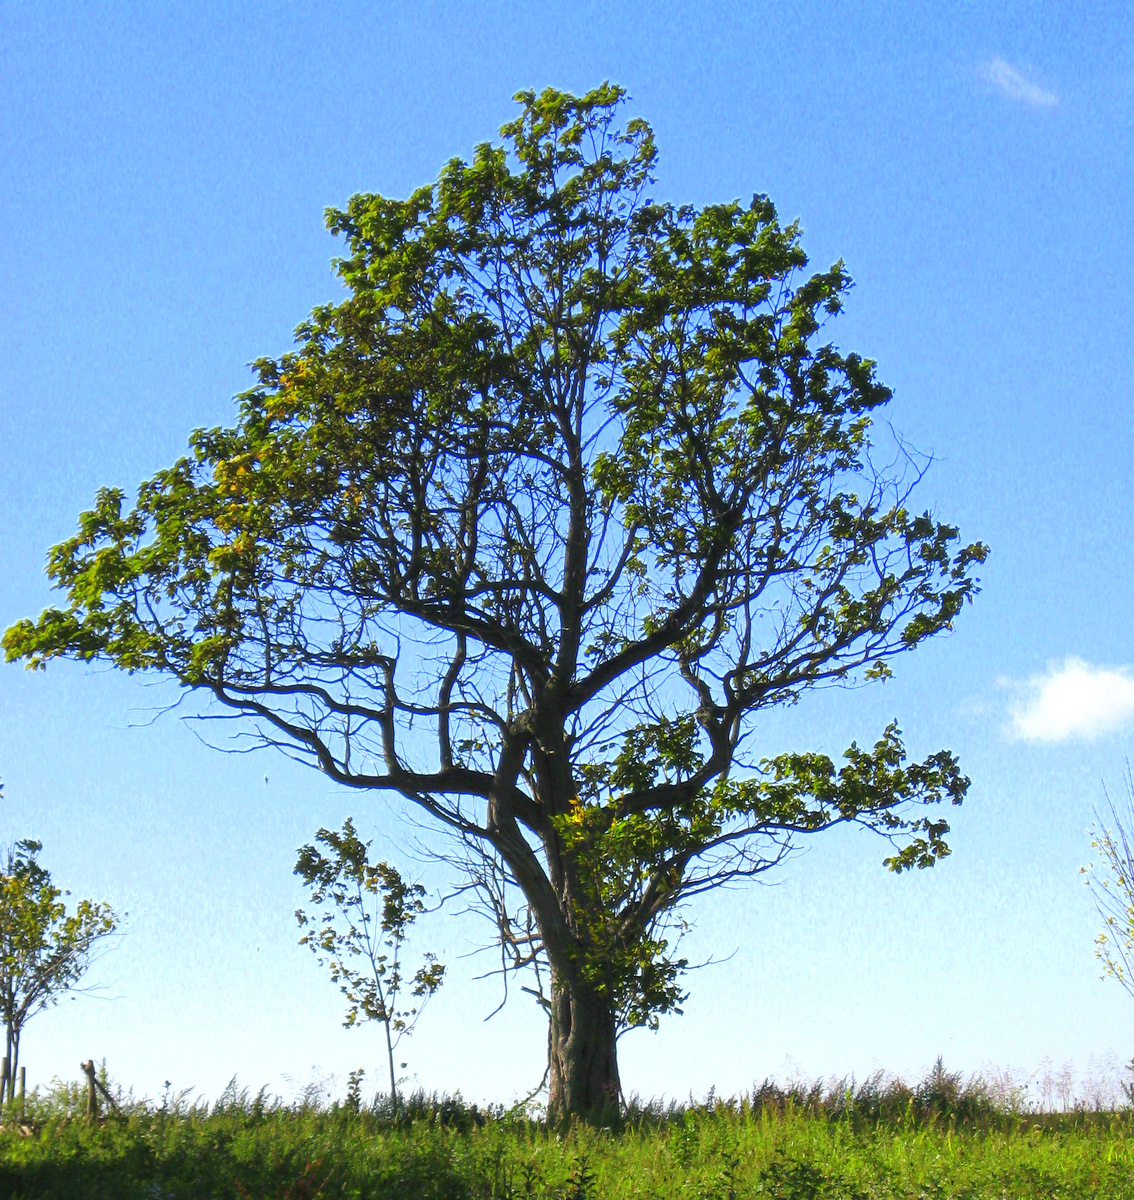
\includegraphics[width=0.5\textwidth,center]{tree.jpg}
            \vspace{-0.8cm}
            \hspace*{6cm}
            \href{https://www.flickr.com/photos/aspis7/5075169756/}
                 {\color{white}\fontsize{5pt}{0}\selectfont @aspis7}
        }
        \only<2>{
            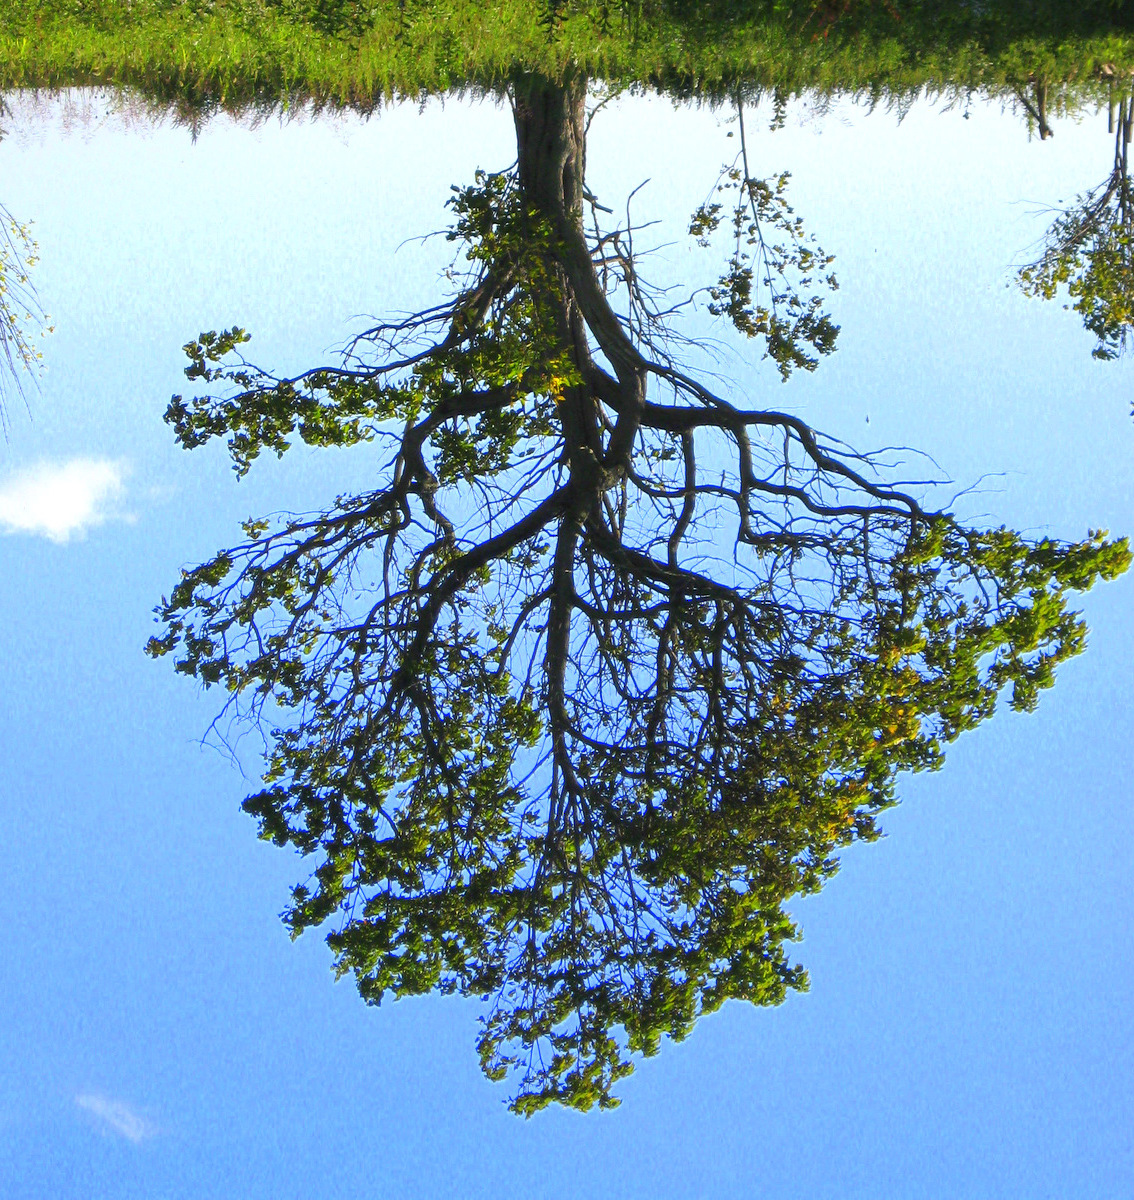
\includegraphics[width=0.5\textwidth,center]{cs_tree.jpg}
            \vspace{-0.8cm}
            \hspace*{6cm}
            \href{https://www.flickr.com/photos/aspis7/5075169756/}
                 {\color{white}\fontsize{5pt}{0}\selectfont @aspis7}
        }
    \end{center}
\end{frame}

\begin{frame}[fragile]{}
    \frametitle{}

    \begin{itemize}[label={\MVRightarrow}]
        \item <+-> Graefe, Goetz and Harumi A. Kuno. “Modern B-tree
            techniques.” IEEE 27th International Conference on Data
            Engineering, 2011.
        \item <+-> D. Comet, "Ubiquitous B-tree", ACM Comp. Surv., vol. 11, no.
            2, 1979.
    \end{itemize}
\end{frame}

\begin{frame}[fragile]{}
    \frametitle{}

    \def\arraystretch{1.5}
    \begin{tabular}{cccc}
        B-Tree & B$^{+}$-Tree & B$_{link}$-Tree & DP-Tree \\
        wB$^{+}$-Tree & NV-Tree & FP-Tree & FASTFAIR \\
        HiKV & Mass-Tree & Skip List & ART \\
        WORT & CDDS-Tree & Bw-Tree & HOT \\
        KISS-Tree & VAST-Tree & FAST & HV-Tree \\
        UB-Tree & LHAM & MDM & Hybrid B$^{+}$-Tree
    \end{tabular}
\end{frame}

\begin{frame}
    \frametitle{}
    \begin{center}

    \only<1>
    {
        \begin{tikzpicture}[]
            \node [rum-node] (memory) at ( 3, 0) {Mem};
            \node [rum-node] (write) at (-3, 0) {Write};
            \node [rum-node] (read) at ( 0, 3) {Read};
            \draw (read) -- (write) -- (memory) -- (read);
            \begin{scope}[on background layer]
                \fill [gray, opacity=0.2]
                    (read.center) --
                    (write.center) --
                    (memory.center) -- cycle;
            \end{scope}
        \end{tikzpicture}
    }

    \only<2>
    {
        \begin{tikzpicture}[]
            \node [rum-node, fill=greenGood] (memory) at ( 3, 0) {Mem};
            \node [rum-node, fill=redBad] (write) at (-3, 0) {Write};
            \node [rum-node, fill=greenGood] (read) at ( 0, 3) {Read};
            \draw (read) -- (write) -- (memory) -- (read);
            \begin{scope}[on background layer]
                \fill [gray, opacity=0.2]
                    (read.center) --
                    (write.center) --
                    (memory.center) -- cycle;
            \end{scope}
        \end{tikzpicture}
    }

    \only<3>
    {
        \begin{tikzpicture}[]
            \node [rum-extra-node] (complex) at ( 0, -3) {Complexity?};
            \node [rum-node] (memory) at ( 3, 0) {Mem};
            \node [rum-node] (write) at (-3, 0) {Write};
            \node [rum-node] (read) at ( 0, 3) {Read};
            \draw (read) -- (memory) -- (complex) -- (write) -- (read);
            \begin{scope}[on background layer]
                \fill [gray, opacity=0.2]
                    (read.center) --
                    (memory.center) --
                    (complex.center) --
                    (write.center) -- cycle;
            \end{scope}
        \end{tikzpicture}
    }

    \end{center}
\end{frame}

\begin{frame}[fragile]{}
    \frametitle{}

    \begin{center}
    \begin{overprint}[12cm]
        \onslide<1>
        \begin{tikzpicture}[]
            \btreenode{1}{}{btree-hide}{}{}
            \btreenode{2}{below=1cm of node1.south}{btree-hide}{}{}
            \btreenode{3}{below=1cm of node1.south west, xshift=-3cm}{btree-hide}{}{}
            \btreenode{4}{below=1cm of node1.south east, xshift=3cm}{btree-hide}{}{}

            \draw[->, btree-line] (pointer11.south) -- (pointer12.north);
            \draw[->, btree-line] (pointer21.south)
                .. controls ([yshift=-1cm] pointer21) and ([yshift=1cm] pointer14) ..
                (pointer14.north);
            \draw[->, btree-line] (pointer31.south)
                .. controls ([yshift=-1cm] pointer31) and ([yshift=1cm] pointer13) ..
                (pointer13.north);
        \end{tikzpicture}

        \onslide<2>
        \begin{tikzpicture}[]
            \btreenode{1}{}{btree-hide}{btree-branch}{}
            \btreenode{2}{below=1cm of node1.south}{btree-hide}{btree-leaf}{}
            \btreenode{3}{below=1cm of node1.south west, xshift=-3cm}{btree-hide}{btree-leaf}{}
            \btreenode{4}{below=1cm of node1.south east, xshift=3cm}{btree-hide}{btree-leaf}{}

            \draw[->, btree-line] (pointer11.south) -- (pointer12.north);
            \draw[->, btree-line] (pointer21.south)
                .. controls ([yshift=-1cm] pointer21) and ([yshift=1cm] pointer14) ..
                (pointer14.north);
            \draw[->, btree-line] (pointer31.south)
            .. controls ([yshift=-1cm] pointer31) and ([yshift=1cm] pointer13) ..
            (pointer13.north);
        \end{tikzpicture}

        \onslide<3>
        \begin{tikzpicture}[]
            \btreenode{1}{}{}{btree-branch}{}
            \btreenode{2}{below=1cm of node1.south}
                {}{btree-leaf}{show-pointers}
            \btreenode{3}{below=1cm of node1.south west, xshift=-3cm}
                {}{btree-leaf}{show-pointers}
            \btreenode{4}{below=1cm of node1.south east, xshift=3cm}
                {}{btree-leaf}{show-pointers}

            \draw[->, btree-line] (pointer11.south) -- (pointer12.north);
            \draw[->, btree-line] (pointer21.south)
                .. controls ([yshift=-1cm] pointer21) and ([yshift=1cm] pointer14) ..
                (pointer14.north);
            \draw[->, btree-line] (pointer31.south)
                .. controls ([yshift=-1cm] pointer31) and ([yshift=1cm] pointer13) ..
                (pointer13.north);
        \end{tikzpicture}

        \onslide<4>
        \begin{tikzpicture}[]
            \btreenode{1}{}{}{btree-branch}{}
            \btreenode{2}{below=1cm of node1.south}
                {}{btree-leaf}{show-pointers}
            \btreenode{3}{below=1cm of node1.south west, xshift=-3cm}
                {}{btree-leaf}{show-pointers}
            \btreenode{4}{below=1cm of node1.south east, xshift=3cm}
                {}{btree-leaf}{show-pointers}

            \draw[->, btree-line, color=red, line width=2pt] (pointer11.south) -- (pointer12.north);
            \draw[->, btree-line] (pointer21.south)
                .. controls ([yshift=-1cm] pointer21) and ([yshift=1cm] pointer14) ..
                (pointer14.north);
            \draw[->, btree-line] (pointer31.south)
                .. controls ([yshift=-1cm] pointer31) and ([yshift=1cm] pointer13)
                .. (pointer13.north);

            \path
              node[btree-path, below=-0.505 of pointer11.west] (path-pointer1) {}
              node[btree-path, below=-0.505 of pointer32.west] (path-pointer2) {};

            \draw[->, btree-line, color=red, line width=2pt]
                (pointer32.south) -- (heap-pointer32.north);

        \end{tikzpicture}
    \end{overprint}
    \end{center}

\end{frame}

\fontsize{18pt}{18}\selectfont
\begin{frame}
  \vspace*{2.5cm}
  \begin{minipage}[b][\paperheight]{\textwidth}
  \begin{center}

      %\raggedright%
      \linespread{1.0}%
      \usebeamerfont{title}%
      \usebeamercolor[fg]{title}%
      \if@noSmallCapitals%
        Questions?
      \else%
        \scshape{\color{black} Questions?}%
      \fi%
      \vspace*{0.3em}

      \usebeamerfont{subtitle}%
      \fontsize{13pt}{14}\selectfont
      \usebeamercolor[fg]{subtitle}%
        \begin{itemize}[label={}]
            \item {\color{black} \github\ \href{github.com/erthalion}
                                               {\color{black}github.com/erthalion}}
            \item {\color{black} \github\ \href{github.com/erthalion/postgres-bcc}
                                               {\color{black}github.com/erthalion/postgres-bcc}}
            \item {\color{black} \twitter\ @erthalion}
            \item {\color{black} \email\ dmitrii.dolgov at zalando dot de}
            \item {\color{black} \email\ 9erthalion6 at gmail dot com}
        \end{itemize}
      \vspace*{2.5em}%

    \vfill
    \vspace*{2em}
  \end{center}
  \end{minipage}

\end{frame}

\end{document}
